\section{Our Approach}
\label{sec:approach}
%In this section, we describe our neural network based joint model for cross-lingual table linking. We first give an overview of our approach, followed by the method for candidate entity generation. Then we describe translation module in detail. Afterwards, we introduce mention, context and coherence features used in our model respectively. In the last part, we discuss the training process and prediction strategy.



In this section, we describe our joint model for cross-lingual table linking.
%\figref{fig:overview} gives a general view of our neural network based joint model.
\figref{fig:overview} gives a general view of the model.
The reason we call it a ``joint model'' is that
the input of neural network is a mention table $X$ containing all the cells to be linked,
together with one candidate entity table $E$,
%All the mentions in the table will be linked simultaneously.
and the output stands for the relevance score $S(X, E)$.



\noindent
\textbf{Candidate Generation:}
%We use several translation tools to generate candidate English entities for each mention represented in Chinese.
%Without a reliable Chinese knowledge base as the bridge,
we use multiple translation tools to produce a set of possible English translations of the given mention in Chinese.
Afterwards, we use several heuristic rules\footnote{{\scriptsize Heuristic rules consist of 1) exact match of any mention translation; 2) anchor entities of any mention translation in KB; 3) fuzzy match of any mention translation. }} to obtain candidate English entities.

\noindent
\textbf{Embedding and Translation Module:}
typically, a mention contains up to three words,
thus we simply represent it as the average embedding of the words it contains. We train word embeddings and entity embeddings on two corpus of different languages separately. 
To tackle the incompatibility of vector space of different languages, we employ a bilingual translation layer.
%to map embeddings from one language space to another.
Taking the mention embedding $\bi{x}^{(m)}$ in Chinese,
the layers translate it into an English mention embedding $\bi{v}^{(m)}$ through linear transformation:
$\bi{v}^{(m)}=W_t \bi{x}^{(m)} + \bi{b}_t$. Where $W_t$ and $\bi{b}_t$ can be randomly initialized or pre-trained.
%\footnote{{\scriptsize See pre-train details in supplementary}}. 
%where $W_t$ is the translation matrix and $\bi{b}_t$ is the bias. We pre-train the translation parameters by leveraging a small number of bilingual word pairs, 
%$(w^{(ch)}, w^{(en)})$, 
%or call them translation seeds.
%The loss function of pre-train step is defined as follows:
%\begin{equation}
%\label{eqn:translation}
%L(W_{t}, \bi{b}_{t}) = \sum_i \Arrowvert W_{t} \bi{w}_i^{(ch)} + \bi{b}_{t} - %\bi{w}_i^{(en)} \Arrowvert_2.
%\end{equation}
%Refer to \secref{sec:impl-detail} and \secref{sec:exp-setup}
%for detail information of the embedding initialization and translation pre-train.

\begin{figure}[th]
	\centering
	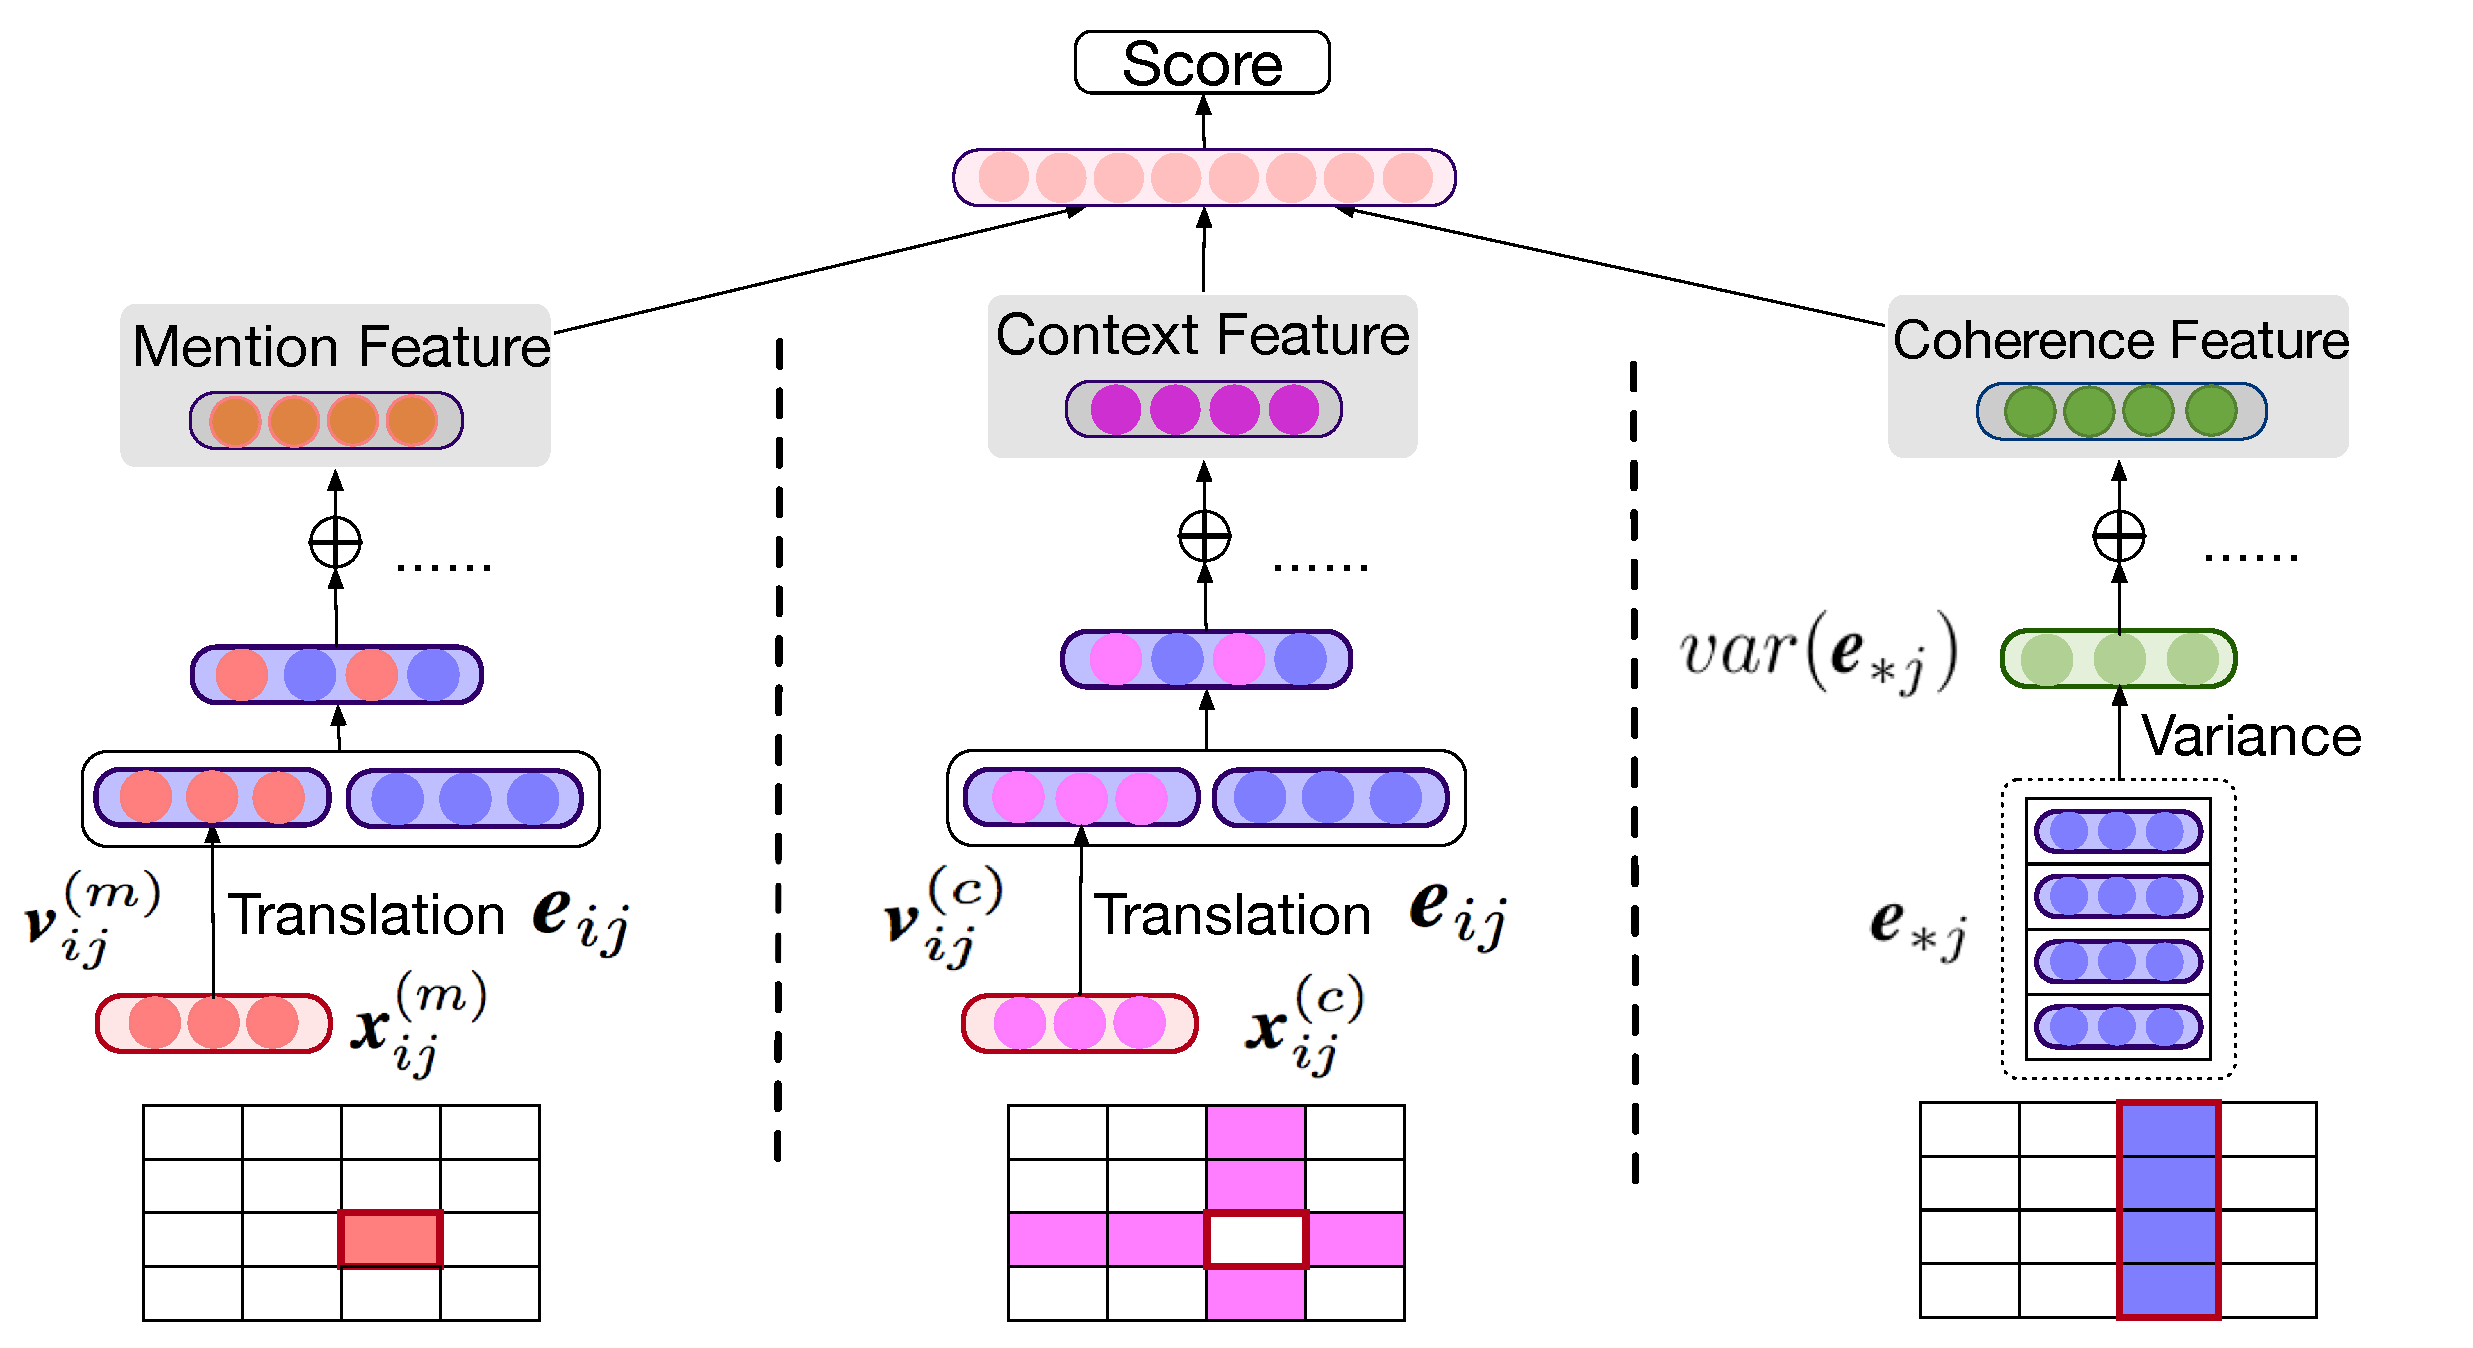
\epsfig{file=figures/overview.eps, angle=0, width=1.0\columnwidth}
	%\scalebox{0.3}{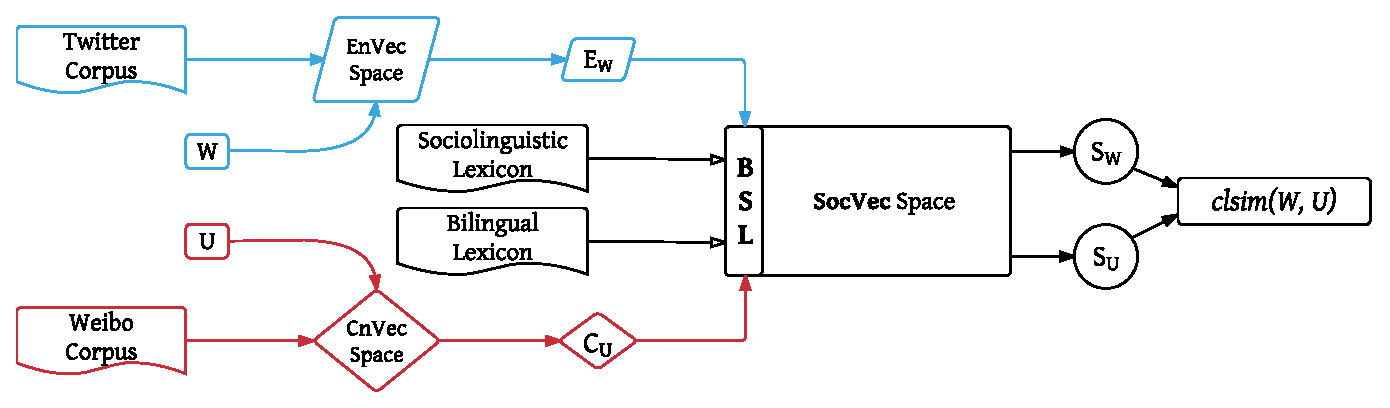
\includegraphics{overview.eps}}
	\caption{Overview of proposed model}
	\label{fig:overview}
\end{figure}

\noindent
\textbf{Mention and Context Feature:}
as shown in \figref{fig:overview}, the mention and context feature represents the relevance or compatiblity between the mention table $X$ and the entity table $E$. We concatenate the translated embedding $\bi{v}_{ij}^{(m)}$ with the entity embedding $\bi{e}_{ij}$, then feed into a fully connected layer,
obtaining the hidden feature between $x_{ij}$ and $e_{ij}$ at mention level.
We apply vector averaging over all cells to be linked
and finally produce the hidden mention feature. 
The context feature follows the similar idea.
Instead of using the surface form $x_{ij}^{(m)}$ itself,
we regard mentions in the same row or column (excluding itself) as the surrounding context and use the average embedding of them, denoted as $x_{ij}^{(c)}$.

\noindent
\textbf{Coherence Feature:}
the inner relationship of entities in the correctly linked table is also valuable. Our intuition is that entities in the same column (row) tend to own the same type.
We calculate the element-wise variance for all entity vectors in the same column
to get a coherence vector for that column.
The average among all columns is the hidden coherence feature of whole entity table.

\noindent
\textbf{Training and Prediction:}
based on the idea of joint model, we construct negative data by randomly corrupting a positive table with different number of cells.
Then we use the pairwise ranking loss to train our model.
In order to reduce the search space at the time of prediction,
we use a local-search descent algorithm to approximate the optimal solution.
%\footnote{{\scriptsize See details in supplementary}}.
